\documentclass[11pt,a4paper]{article}
\usepackage[T1]{fontenc}
\usepackage[utf8]{inputenc}
\usepackage{lmodern}
\usepackage{amsmath,amssymb,amsthm,mathtools,mathrsfs}
\usepackage{graphicx,float,xcolor,multicol}
\usepackage[shortlabels]{enumitem}
\usepackage[margin=27mm]{geometry}
\usepackage{microtype,needspace,placeins}
\usepackage{tikz,tikz-cd}
\usetikzlibrary{arrows.meta,calc,positioning,patterns,decorations.pathreplacing}
\usepackage[colorlinks=true,linkcolor=teal,urlcolor=teal,citecolor=teal]{hyperref}
\setlength{\parindent}{0pt}
\setlength{\parskip}{.6em}
\setcounter{secnumdepth}{0}
\allowdisplaybreaks
\raggedbottom
\providecommand{\cross}{\times}
\DeclareUnicodeCharacter{2020}{\ensuremath{\dagger}}
\DeclareMathOperator{\supp}{supp}
\DeclareMathOperator*{\esssup}{ess\,sup}
\providecommand{\chapter}{\section}
\newenvironment{tool}[2]{\subsection*{Tool #1 --- #2}}{}
\newcommand{\ToolRef}[1]{Tool #1}
\newcommand{\FigureTag}[2]{\textit{Figure #1}}
\newcommand{\Result}[1]{\subsection*{#1}}
\newcommand{\Application}[1]{\subsubsection*{Application\if\relax\detokenize{#1}\relax\else\space--- #1\fi}}
\newcommand{\ProofHeading}{\par\textit{Proof.}\space}
\newcommand{\ProofOf}[1]{\par\textit{Proof of #1.}\space}
\newcommand{\RemarkHeading}{\par\textbf{Remark.}\space}
\newcommand{\NoteHeading}{\par\textbf{Note.}\space}
\newcommand{\ExerciseHeading}{\par\textbf{Exercise.}\space}

\graphicspath{{figures/complex-analysis/}}
\begin{document}
\section*{Harmonic Functions and Rectifiable Curves}
% BLOG-CONTENT-BEGIN
Let us apply the epsilon-room method to harmonic functions.

Let $u\colon U\to\mathbb R$ be harmonic, that is,
\[
\Delta u:=\frac{\partial^2u}{\partial x^2}
+\frac{\partial^2u}{\partial y^2}=0,
\]
and let $K\subset U$ be compact. Then
\[
\sup_{z\in K}u(z)=\sup_{z\in\partial K}u(z).
\]
This is the maximum principle for harmonic functions.

\textit{Proof.}
Since $\partial K\subseteq K$, as $K$ is compact,
\[
\sup_{z\in K}u(z)\geq\sup_{z\in\partial K}u(z).
\]
We shall show that strict inequality can never occur. Suppose it does. Then $u$ attains a maximum in $\operatorname{int}(K)$, say at
\[
z_0\in\operatorname{int}(K).
\]
Let $B_\varepsilon(z_0)\subset\operatorname{int}(K)$, where $z_0=x_0+iy_0$. Consider the restriction
\[
x\longmapsto u(x+iy_0),
\qquad x\in[x_0,x_0+\varepsilon/2].
\]
The second derivative test gives
\[
\frac{\partial^2u}{\partial x^2}(z_0)\leq0.
\]
Similarly, \(\frac{\partial^2u}{\partial y^2}(z_0)\leq0.\)
Since $u$ is harmonic, both must be equalities. We intend to contradict this, so let us give $u$ some $\varepsilon$-room. Define
\[
\boxed{u_\varepsilon(x+iy):=u(x+iy)+\varepsilon(x^2+y^2).}
\]


Suppose
\[
\sup_{z\in K}u(z)>\sup_{z\in\partial K}u(z).
\]
Then there is an $\varepsilon'>0$ such that
\[
\sup_{z\in K}u(z)>
\sup_{z\in\partial K}u(z)+\varepsilon'.
\]
The function $x^2+y^2$ is continuous on $K$. Let
\[
\sup_{x+iy\in K}(x^2+y^2)=M,
\]
and set $\varepsilon=\varepsilon'/M$. Then
\[
\sup_{z\in\partial K}u_\varepsilon(z)
<\sup_{z\in\partial K}u(z)+\frac{\varepsilon'}{M}M
<\sup_{z\in K}u(z)
<\sup_{z\in K}u_\varepsilon(z).
\]
Thus $u_\varepsilon$ again has an interior maximum, and
\[
\frac{\partial^2u_\varepsilon}{\partial x^2}\leq0,
\qquad
\frac{\partial^2u_\varepsilon}{\partial y^2}\leq0.
\]
Adding these inequalities gives \(4\varepsilon\leq0,\)
a contradiction. Therefore
\[
\boxed{
\sup_{z\in K}u(z)=\sup_{z\in\partial K}u(z).}
\]

\textbf{Note.}
If $f\colon U\to\mathbb C$ is holomorphic, then \(\operatorname{Re}(e^{i\theta}f)\)
is harmonic, and
\[
\sup_{z\in K}\operatorname{Re}(e^{i\theta}f)
=\sup_{z\in\partial K}\operatorname{Re}(e^{i\theta}f)
\qquad(\forall\theta\in[0,2\pi)).
\]
Hence
\[
\sup_{z\in K}\sup_\theta\operatorname{Re}(e^{i\theta}f)
=\sup_{z\in\partial K}\sup_\theta\operatorname{Re}(e^{i\theta}f).
\]
By Tool 2, this yields
\[
\sup_{z\in K}|f(z)|=\sup_{z\in\partial K}|f(z)|.
\]
As was stated, a fact about real-valued functions is lifted to a complex-valued function via Tool 2.

\textbf{Exercise.}
The only infima of $|f|$ attained in the interior for a holomorphic function occur at zeros of the function.


The following is a generalized form of the $\varepsilon$-technique.

The image of a rectifiable curve has measure $0$.

\textbf{Remark.}
Space-filling curves are not rectifiable. In fact, any curve with Hausdorff dimension greater than $1$ is unrectifiable.

The picture below shows that Riemann-integrable functions have graphs of measure $0$.

\begin{figure}[htbp]
  \centering
  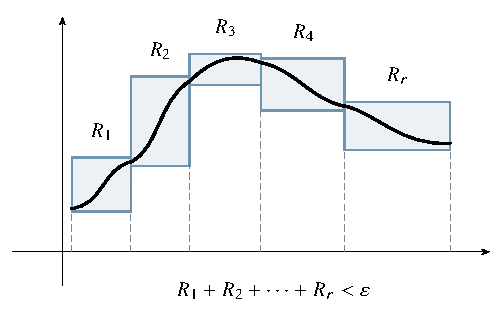
\includegraphics[width=0.72\linewidth]{note2-fig-01.pdf}

\end{figure}

In particular, graphs of continuous or almost-continuous functions also have measure $0$. If we invoke Littlewood's principle, namely Lusin's theorem, then the graph of any measurable function whose support is a set of finite measure has measure $0$, since such functions are ``almost'' continuous. Sadly, none of these capture the notion of rectifiability, since there is no implicit function theorem for continuous functions.



\subsection*{Tool 6 — Fundamental Theorem of Calculus}
Let $f$ be Riemann integrable, and let $F$ satisfy $F'=f$. Then
\[
\int_a^b f(x)\,dx=F(b)-F(a).
\]


Let $u\colon U\to\mathbb R$ be harmonic on a simply connected region $U$. Then there is a harmonic function $v\colon U\to\mathbb R$, unique up to constants and called the harmonic conjugate, such that $u+iv$ is holomorphic in $U$.

\textit{Proof.}
If $u$ is harmonic, then \(u_x-iu_y\)
is holomorphic, since
\[
u_{xx}=-u_{yy},
\qquad
u_{xy}=-(-u_{yx}).
\]
Now, if $u\colon U\to\mathbb R$ and $U$ is simply connected, then $g(z):=u_x-iu_y$ has a primitive. Let that primitive be $f(z)$. The Wirtinger derivative satisfies
\begin{align*}
\frac{\partial f}{\partial z}
=f'(z)
=g(z)
&=u_x-iu_y\\
&=\operatorname{Re}(f)_x-i\operatorname{Re}(f)_y.
\end{align*}
Therefore
\[
\operatorname{Re}(f)_x=u_x,
\qquad
\operatorname{Re}(f)_y=u_y,
\]
so \(u=\operatorname{Re}(f)+c.\) After adjusting the constant term of $f$, we may take $c=0$.
Thus $\operatorname{Im}(f)$ is the required conjugate.

\textbf{Remark.}
Let $f\colon\mathbb C\to\mathbb R$ be harmonic and holomorphic, viewing it also as a complex-valued function. Then $0$ is a harmonic conjugate of $\operatorname{Re}(f)$. By the fundamental theorem of calculus, one concludes that $\operatorname{Re}(f)$ is constant, and hence $f$ is constant. Thus holomorphic functions demand more than one dimension to be harmonic, but, as it turns out, they do not merely demand it: they ensure that they get multidimensional freedom; they ensure harmony. In fact, they turn out to be smooth.


\textbf{Remark.}
Suppose $u$ and $v$ are harmonic and defined on all of $\mathbb C$. Let \(u\leq v+M.\)
Then $u-v$ is harmonic and $u-v\leq M$. Let $w$ be its harmonic conjugate. Then
\[
(u-v)+iw
\]
is entire, so \(e^{(u-v)+iw}\)
is entire and bounded. Hence
\[
u=v+k.
\]
If equality in $u\leq v+M$ is attained, then $u=v+M$. ``A function in harmony never dominates another of the same kind.'' The same argument shows that an entire function with bounded real part is constant.
% BLOG-CONTENT-END
\end{document}
